\documentclass[../main.tex]{subfiles}
\begin{document}
%=========================================TRUYỆN CHÍNH========================================
\subsection*{1. Image Captioning là gì?}
\addcontentsline{toc}{subsection}{Image Captioning là gì?}

Image Captioning (hay thuật toán sinh văn bản dựa theo ảnh) là một thuật toán giúp máy tính sinh ra một đoạn văn bản mô tả một ảnh. Đây là một bài toán trong lĩnh vực xử lý ngôn ngữ tự nhiên (Natural Language Processing, NLP) và được ứng dụng rộng rãi trong các ứng dụng như dịch thuật, tìm kiếm hình ảnh, đánh giá hình ảnh, dịch thuật, v.v.

Thuật toán này thực hiện nhiệm vụ dự đoán chú thích cho một hình ảnh nhất định dựa theo các đặc điểm thuộc tính có trong bức ảnh. Các ứng dụng phổ biến trong thế giới thực của nó bao gồm hỗ trợ người khiếm thị có thể giúp họ điều hướng qua các tình huống khác nhau. Do đó, chú thích hình ảnh giúp cải thiện khả năng tiếp cận nội dung cho mọi người bằng cách mô tả hình ảnh cho họ.

Theo đó, thuật toán này gồm input-output như sau:

\begin{itemize}
    \item Input: Một hình ảnh;
    \item Output: Một chuỗi các từ mô tả hình ảnh dựa theo các đặc điểm.
\end{itemize}

\subsection*{2. Ứng dụng}
\addcontentsline{toc}{subsection}{Ứng dụng}

Image Captioning (tạo chú thích hình ảnh tự động) có nhiều ứng dụng thiết thực trong đời sống, công nghệ và nghiên cứu, bao gồm:

\begin{enumerate}
    \item \textbf{Hỗ trợ người khiếm thị:} Mô tả hình ảnh tự động giúp người khiếm thị hiểu nội dung ảnh thông qua giọng nói (screen reader).

    Ví dụ: Ứng dụng như Seeing AI (Microsoft) sử dụng AI để mô tả cảnh vật, chữ viết, cảm xúc.

    \item \textbf{Tìm kiếm hình ảnh thông minh:} Cải thiện kết quả tìm kiếm bằng cách hiểu nội dung ảnh thay vì chỉ dựa vào metadata hoặc tags.

    Ví dụ: Google Images sử dụng AI để phân tích và gán nhãn ảnh.

    \item \textbf{Mạng xã hội \& Nền tảng chia sẻ ảnh:} Tự động gợi ý chú thích (caption) cho ảnh đăng tải trên Facebook, Instagram.

    Ví dụ: Phát hiện nội dung không phù hợp (ảnh bạo lực, ảnh hưởng xấu).

    \item \textbf{Y tế \& Chẩn đoán hình ảnh:} Mô tả tự động kết quả X-quang, MRI, CT scan để hỗ trợ bác sĩ.

    Ví dụ: AI mô tả tổn thương trong ảnh y tế.

    \item \textbf{Giáo dục \& Học tập:} Tạo mô tả cho hình ảnh trong sách giáo khoa, tài liệu học tập.

    Ví dụ: Hỗ trợ học ngoại ngữ (ghép ảnh với từ vựng).

    \item \textbf{An ninh \& Giám sát:} Tự động mô tả sự kiện trong camera an ninh.

    Ví dụ: Phát hiện hành vi đáng ngờ qua phân tích hình ảnh.

    \item \textbf{Thương mại điện tử:} Tự động gán nhãn sản phẩm từ ảnh ("Áo thun màu xanh, chất cotton").

    Ví dụ: Pinterest sử dụng AI để đề xuất sản phẩm tương tự.

    \item \textbf{Robot \& Xe tự lái:} Giúp robot/xe tự lái "hiểu" môi trường xung quanh qua mô tả bằng ngôn ngữ.

    Ví dụ: Tesla sử dụng AI để nhận diện vật thể và cảnh báo nguy hiểm.
\end{enumerate}

\subsection*{3. Các mô hình phổ biến}
\addcontentsline{toc}{subsection}{Các mô hình phổ biến}

Trong thế giới hiện tại, có nhiều mô hình Image Captioning được phát triển và áp dụng, trong đó có những mô hình được sử dụng phổ biến như:

\begin{enumerate}
    \item Mô hình dựa trên CNN và LSTM: đây là các mô hình dạng cổ điển và được sử dụng phổ biến nhất. Mô hình này sử dụng CNN để trích xuất đặc trưng từ ảnh và LSTM để sinh ra chú thích. Trong đó:
    \begin{itemize}
        \item Show and Tell (2015)
        \begin{itemize}
            \item Kiến trúc: CNN + LSTM
            \item Ý tưởng: dùng CNN làm encoder, LSTM làm decoder.
            \item Ưu điểm: đơn giản, hiệu quả với dữ liệu nhỏ.
        \end{itemize}

        \item Show, Attend and Tell (2015)
        \begin{itemize}
            \item Bổ sung cơ chế Attention để tập trung vào vùng ảnh quan trọng khi sinh từng từ.
            \item Ưu điểm: Cải thiện độ chính xác cho ảnh phức tạp.
        \end{itemize}

        \item NIC (Neural Image Captioning) (2015)
        \begin{itemize}
            \item Kiến trúc: CNN + LSTM, ngoại trừ việc nó sử dụng ResNet (hoặc VGG16) làm encoder thay vì CNN thông thường.
            \item Ứng dụng tốt cho Flickr8k, Flickr30k.
        \end{itemize}
    \end{itemize}
    \item Mô hình dựa trên Transformer: đây là các mô hình mới và được phát triển gần đây. Mô hình này sử dụng kiến trúc Transformer để sinh ra chú thích. Trong đó:
        \begin{itemize}
            \item Vision Transformer + Transformer Decoder (2020)
            \begin{itemize}
                \item Kiến trúc: CNN + Transformer
                \item Encoder: ViT chia ảnh thành các patch và mã hóa thành các token.
                \item Decoder: Transformer sinh caption dựa trên token ảnh.
                \item Ưu điểm: Hiệu suất cao với dữ liệu lớn.
            \end{itemize}
            \item OFA (One For All) (2021)
            \begin{itemize}
                \item Đa nhiệm: Unified model cho Image Captioning, VQA, Text-to-Image.
                \item Kiến trúc: Transformer, các patch được huân luyện trước có thể sử dụng trên đa dạng tác vụ.
            \end{itemize}
            \item BLIP (Bootstrap Language-Image Pre-training) (2022)
            \begin{itemize}
                \item Kết hợp CLIP và GPT: Vừa hiểu ảnh, vừa sinh văn bản mạch lạc.
                \item Ứng dụng: Tạo caption chất lượng cao, chỉnh sửa caption.
            \end{itemize}
            \item GIT (GenerativeImage2Text) (2022)
            \begin{itemize}
                \item Tận dụng Vision Transformer (ViT) và Transformer Decoder.
                \item Đặc điểm: Huấn luyện trên lượng dữ liệu khổng lồ (hàng tỷ ảnh)
            \end{itemize}
            \end{itemize}
    \item Ngoài ra còn có các mô hình khác như VinVL (Sử dụng CNN và Transformer), hay CoCa (Contrastive Captioners).
\end{enumerate}

\subsection*{4. Các kiến thức liên quan}
\addcontentsline{toc}{subsection}{Các kiến thức liên quan}

\subsubsection*{4.1 CNN}
\addcontentsline{toc}{subsubsection}{CNN}

CNN (Convolutional Neural Network) là một loại mạng nơ-ron tích chập được sử dụng phổ biến trong xử lý ảnh và nhận dạng hình ảnh. Chúng được thiết kế để trích xuất đặc trưng từ ảnh bằng cách áp dụng các lớp tích chập và các lớp tổng hợp.

\begin{figure}[H]
    \centering
    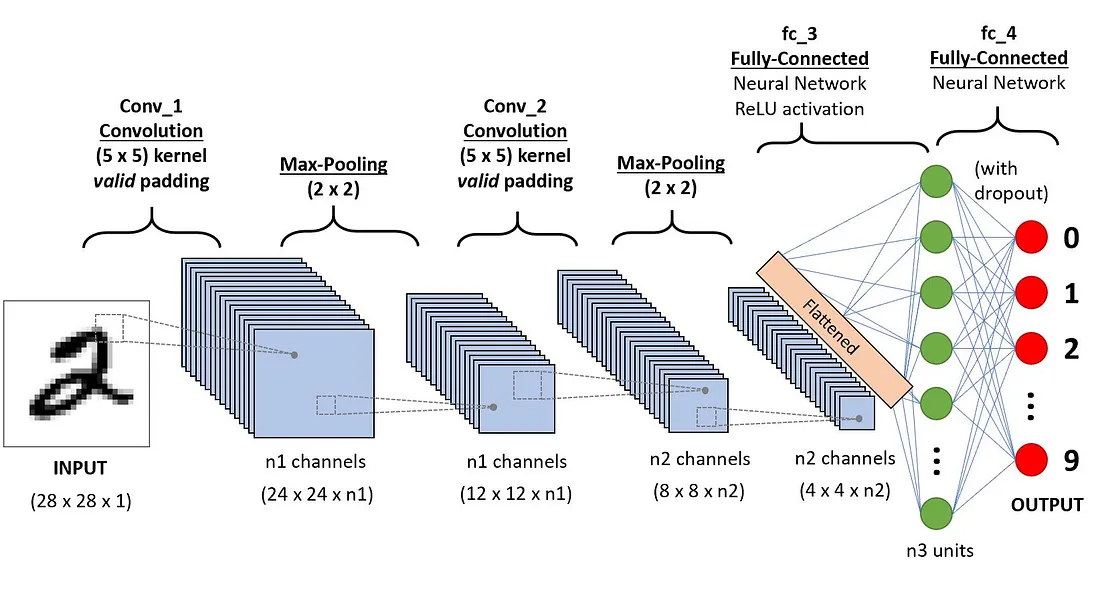
\includegraphics[width=0.5\textwidth]{Image/CNN.png}
    \caption{CNN}
    \label{fig:CNN}
\end{figure}

\subsubsection*{4.2 RNN}
\addcontentsline{toc}{subsubsection}{RNN}

RNN (Recurrent Neural Network) là một loại mạng nơ-ron có trạng thái được sử dụng phổ biến trong xử lý ngôn ngữ tự nhiên và xử lý chuỗi thời gian. RNN được thiết kế để xử lý chuỗi dữ liệu có tính tuần tự, trong đó mỗi phần tử của chuỗi được xử lý dựa trên thông tin từ phần tử trước đó.

\begin{figure}[H]
    \centering
    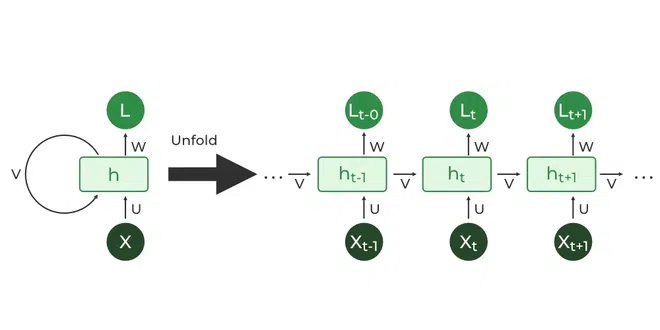
\includegraphics[width=0.5\textwidth]{Image/RNN.png}
    \caption{RNN}
    \label{fig:RNN}
\end{figure}

\subsubsection*{4.3 LSTM}

LSTM (Long Short-Term Memory) là một loại mạng nơ-ron có trạng thái được sử dụng phổ biến trong xử lý ngôn ngữ tự nhiên và xử lý chuỗi thời gian. LSTM được thiết kế để xử lý chuỗi dữ liệu có tính tuần tự, trong đó mỗi phần tử của chuỗi được xử lý dựa trên thông tin từ phần tử trước đó.

\begin{figure}[H]
    \centering
    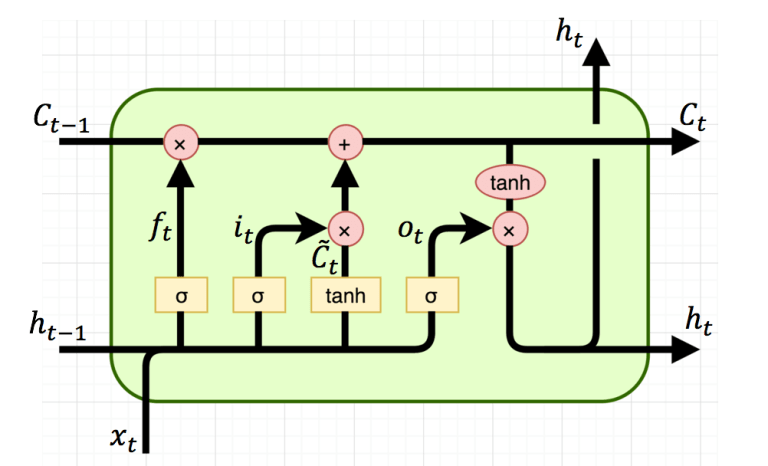
\includegraphics[width=0.5\textwidth]{Image/lstm.png}
    \caption{RNN}
    \label{fig:RNN}
\end{figure}

Điểm khác biệt giữa LSTM và RNN là LSTM có thể lưu trữ thông tin dài hạn hơn so với RNN thông qua các cổng ghi và đọc. Điều này giúp LSTM có thể xử lý chuỗi dữ liệu có độ dài lớn hơn so với RNN.

\subsubsection*{4.4 Mô hình CLIP}
\addcontentsline{toc}{subsubsection}{Mô hình CLIP}

CLIP (Contrastive Language-Image Pre-training) là một mô hình học sâu được thiết kế để học cách biểu diễn hình ảnh và văn bản bằng cách so sánh chúng với các cặp ảnh-đoạn văn bản. Mô hình này được huấn luyện trên một tập dữ liệu lớn và được sử dụng để học cách biểu diễn hình ảnh và văn bản trong không gian vector.

\end{document}